\documentclass[11pt, a4paper, landscape]{article}
\usepackage[english,userlastpage,triangle,utf-8]{NeyDreuwSlides_Oct08}
\usepackage{algorithm}
\usepackage{algpseudocode}
\usepackage{tikz}
\usepackage{pifont}
\usepackage{wasysym}
\usepackage{amssymb}
\usepackage{pdfpages}
\usepackage{color}

\renewcommand*{\title}{ASR Lab Results}                               % main title of the work (used for \TitlePage)
\renewcommand*{\titleshort}{ASR Lab Results}                    % short title (used for \lfoot)
\renewcommand*{\occasion}{Presentation} % (used for \TitlePage)
\renewcommand*{\occasionshort}{~}  % short occasion title (used for \rfoot)
\renewcommand*{\date}{\today}
\renewcommand*{\author}{Ilya Sklyar, Konstantin Kromberg, Miguel Gra\c{c}a}                                     % all the authors of the work, can be long (used for \TitlePage)
\renewcommand*{\authorshort}{Sklyar, Kromberg, Gra\c{c}a~~}                                        % all the authors of the work, should be short (used for \lfoot)
\renewcommand*{\email}{~}             % all email address(es) of the authors (used for \TitlePage)
\renewcommand*{\mainauthor}{Ilya Sklyar, Konstantin Kromberg, Miguel Gra\c{c}a}                                 % the author(s) who presented the work (used for \FinalPage)
\renewcommand*{\mainauthoremail}{\email}                                  % presenter mail address(es) (used for \FinalPage)
\renewcommand*{\www}{~}            % web address (used for \TitlePage _and_ \FinalPage)
\newcommand*{\keywords}{Title of Presentation, etc.}      % keywords for pdf summary
\renewcommand{\arraystretch}{1.2}

% will be set into the PDF document summary
\hypersetup{
  pdftitle={\title}, 
  pdfsubject={\occasion},  
  pdfauthor={\author}, 
  pdfkeywords={\keywords}
}

%%%%%%%%%%%%%%%%%%%%%%%%%%%%%%%%%%%%%%%%%%%%%%%%%%%%%%%%%%%%%%%%%%%%%%%%%%%%%%%%
\usepackage[insection]{minitoc}
\renewcommand{\stifont}{\normalsize\bf} 
\renewcommand{\stcfont}{\normalsize\bf}
\renewcommand{\stcSSfont}{\normalsize\bf}

\begin{document}

%%%%%%%%%%%%%%%%%%%%%%%%%%%%%%%%%%%%%%%%%%%%%%%%%
\TitlePage

%%%%%%%%%%%%%%%%%%%%%%%%%%%%%%%%%%%%%%%%%%%%%%%%%
\NewPage\headline{Overview}
\vfill
\begin{itemize}
  \item Gaussian Mixture Model (GMM) Tuning
  \begin{itemize}
    \item Expectation-Maximization (EM) Parameters
    \item Alignment Parameters
    \item Search Results
  \end{itemize}
  \item Neural Network (NN) Tuning
  \begin{itemize}
    \item Write stuff here
    \item Search Results
  \end{itemize}
  \item Testing Environment
\end{itemize}
\vfill

%%%%%%%%%%%%%%%%%%%%%%%%%%%%%%%%%%%%%%%%%%%%%%%%%
\NewPage\headline{GMM Tuning: EM Parameters}
\vfill
Basic setup:
\begin{itemize}
  \item Lexicon consists of 106 states
  \item Exact computation of the linear segmentation
  \item Maximum approximation for GMMs
  \item 6 EM steps
  \item 4 density splits
\end{itemize} 
\vspace{20pt}
Tunable properties:
\begin{itemize}
  \item Minimum observations per density
  \item Pooling type
\end{itemize}
\vspace{20pt}
Tuning is based on the likelihood of the training data
\vfill

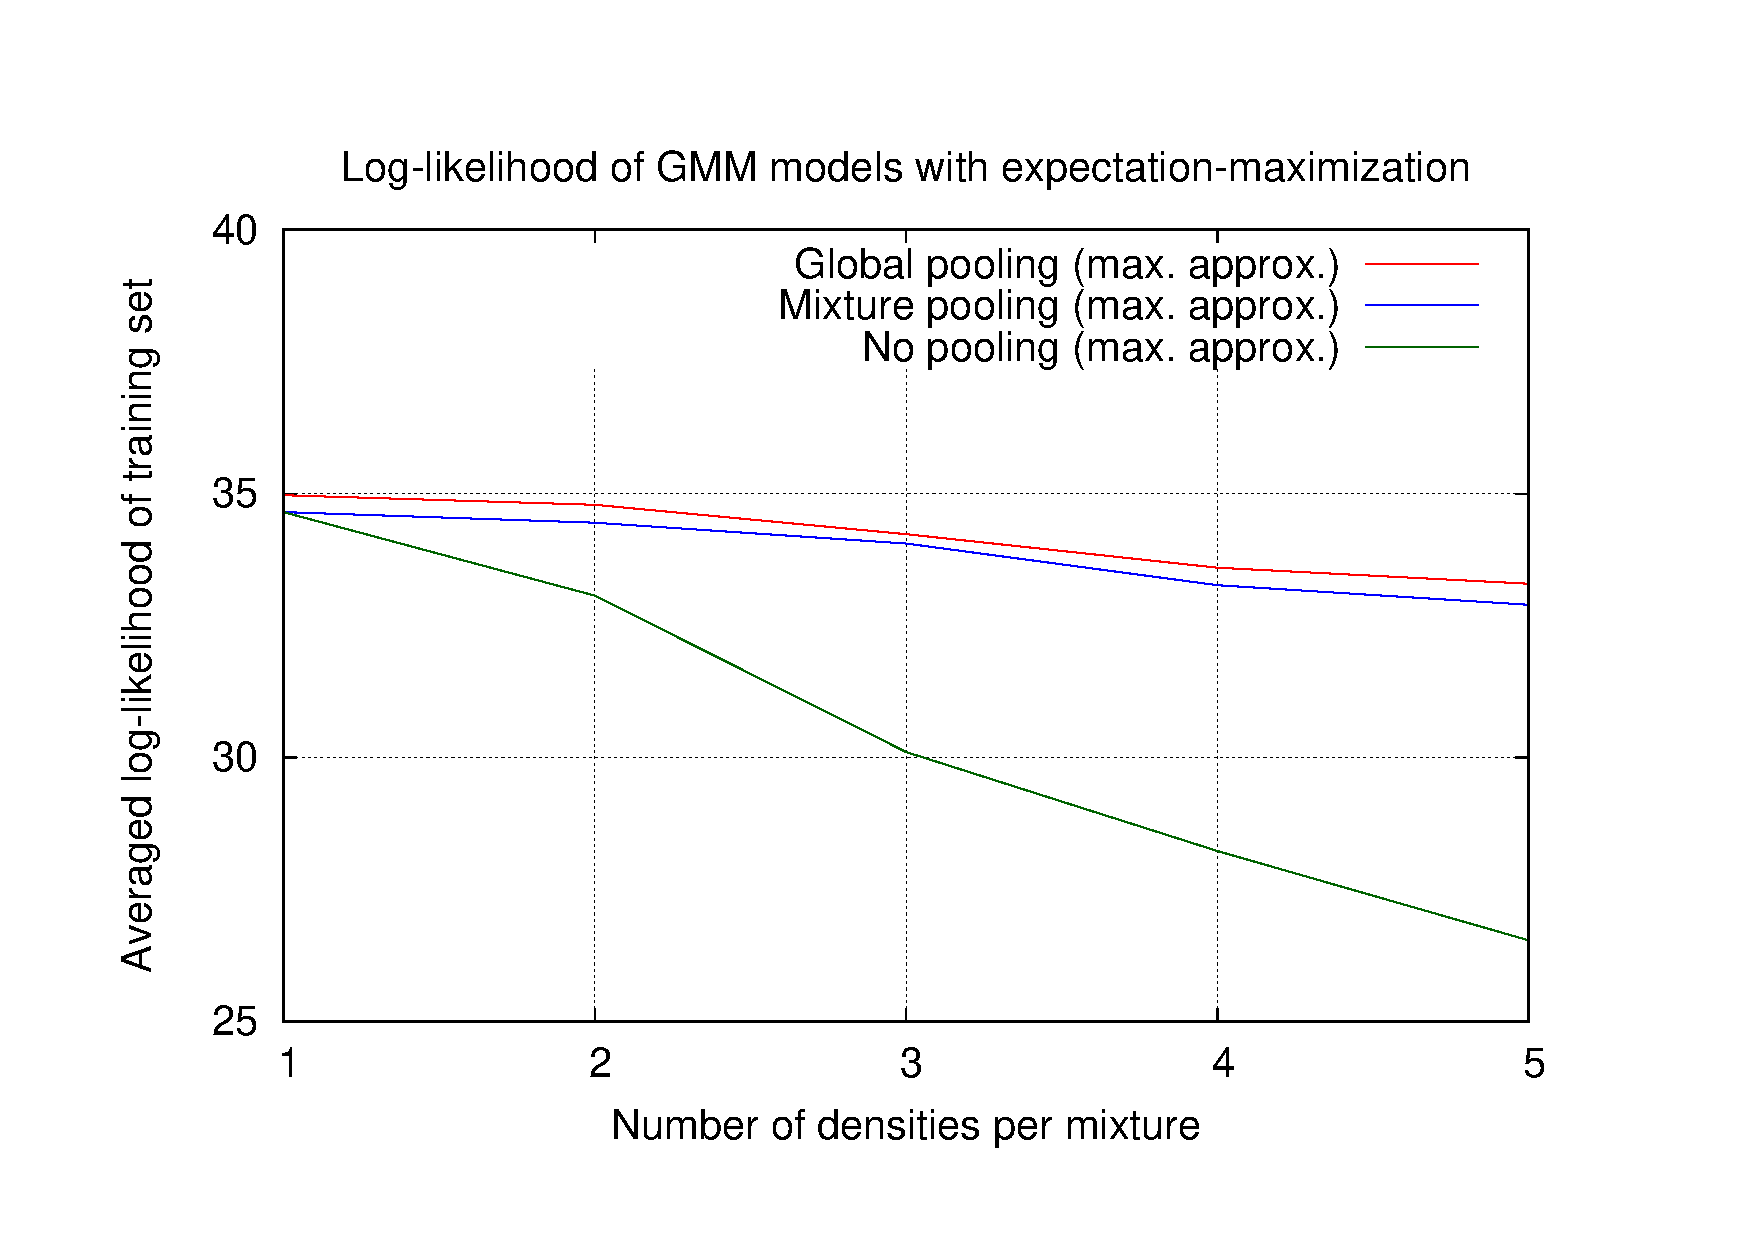
\includepdf[pages=-]{plots/am_score_afterSplit.pdf} 

%%%%%%%%%%%%%%%%%%%%%%%%%%%%%%%%%%%%%%%%%%%%%%%%%%%
\NewPage\headline{GMM Tuning: EM Parameters}
\vfill
Pooling:
\begin{itemize}
	\item No pooling results in better model fitting than using pooling 
	\item Global and mixture-level pooling perform similarly 
  \item Due to the size of the data, there is little reason to use pooling
\end{itemize}
\vspace{20pt}
Splitting criterion:
\begin{itemize}
	\item Minimum number of observations per density has a small influence
	\item Sufficient data points per density in a mixture due to:
	\begin{itemize}
		\item At most $5$ densities per mixture
		\item Each density has, in average, $7$K data points.
	\end{itemize}
\end{itemize}
\vfill

%%%%%%%%%%%%%%%%%%%%%%%%%%%%%%%%%%%%%%%%%%%%%%%%
\NewPage\headline{GMM Tuning: Alignment Parameters}
\vfill
Tunable parameters (optimized on the best performing EM setup):
\begin{itemize}
	\item Time distortion penalty (TDP) values:
    \begin{itemize}
      \item Forward transitions do not have costs (to enforce monotonicity)
      \item Skip and loop transitions have differing costs
      \item Due to high number of states per word, skips should cost more
    \end{itemize}
	\item Pruning threshold
\end{itemize}
\vfill

%%%%%%%%%%%%%%%%%%%%%%%%%%%%%%%%%%%%%%%%%%%%%%%%
\NewPage\headline{Alignment Results}
\vfill
\begin{itemize}
  \item Evaluation on acoustic model (AM) score and silence ratio in resulting alignment
  \item Pruning threshold set to 200 (run with higher thresholds)
  \item TDP format (Loop-Forward-Skip) 
\end{itemize}

\begin{center}
\begin{tabular}{| l |  c | c |} \toprule
  TDP values & AM score           & Silence [\%]      \\ \midrule
  1-0-10     & \color{red}{22.68} & \color{red}{43.48}\\
  2-0-20     & 22.73              & 53.20             \\
  3-0-30     & 23.05              & 59.60             \\ \midrule
  10-0-10    & 23.98              & 75.61             \\
  20-0-20    & 24.31              & 80.35             \\
  30-0-30    & 24.37              & 80.35             \\ \bottomrule
\end{tabular}
\end{center}
\begin{itemize}
	\item Cheaper loop transitions results in alignments with less silence
	\item First 3 systems have similar AM scores, but differing silence ratios
\end{itemize}
\vfill


%%%%%%%%%%%%%%%%%%%%%%%%%%%%%%%%%%%%%%%%%%%%%%%%
\NewPage\headline{Search Results}
\vfill
\begin{itemize}
	\item Optimization performed on the first 1000 segments of test corpus
	\item Tuning: Word penalty (WP) and TDP depending on word error rate (WER)
	\item \color{red}{no need to show SER and RTF if you tune on WER and RTF is not given in seconds. It's a ratio :)}
\end{itemize}

\begin{center}
	\begin{tabular}{| l | c | c | c |} \toprule
		WP/TDP      &    WER [\%]    & SER [\%]    & RTF [s]    \\ \midrule
		80/1-0-10   &    5           &    13       & 0.026      \\
		80/2-0-20   &\color{red}{4.2}&    11.1     & 0.039      \\
		80 /3-0-30  &    4.27        &    11.4     & 0.044      \\ \midrule
		80 /10-0-10 &    7.11        &    19.5     & 0.052      \\
		100/20-0-20 &    22.56       &    52.5     & 0.048      \\
		120/30-0-30 &    36.54       &    74.8     & 0.041      \\ \bottomrule
		
	\end{tabular}
\end{center}
Results for whole corpus 80/2-0-20:
\begin{itemize}
	\item WER: 4.63\% SER: 12.03\%  RTF: 0.37
\end{itemize}
\vfill

%%%%%%%%%%%%%%%%%%%%%%%%%%%%%%%%%%%%%%%%%%%%%%%%%
\NewPage\headline{Testing Environment}
\vfill
Hardware:
\begin{itemize}
  \item Intel i5-4690K @ 3.5GHz, Quad Core, SSE2 registers
  \item 16GB DDR3 1333MHz RAM
\end{itemize}

\begin{table}[]
\centering
\textbf{
\begin{tabular}{l | c | c | c } \toprule
Pipeline step & Time(s) 1 thread & Time(s) 4 threads & RTF \\ \midrule
GMM Training  &                  &                   &     \\
GMM Search    &                  &                   &     \\ \midrule
NN Training   &                  &                   &     \\
NN Search     &                  &                   &     \\ \bottomrule
\end{tabular}
}
\end{table}
\vfill

%%%%%%%%%%%%%%%%%%%%%%%%%%%%%%%%%%%%%%%%%%%%%%%%
\NewPage\headline{Last week}
\vfill
\vfill

%%%%%%%%%%%%%%%%%%%%%%%%%%%%%%%%%%%%%%%%%%%%%%%%
\NewPage\headline{Last week}
\vfill
\vfill

%%%%%%%%%%%%%%%%%%%%%%%%%%%%%%%%%%%%%%%%%%%%%%%%
\NewPage\headline{Last week}
\vfill
\vfill
\FinalPage
\end{document}
